 

\documentclass[12pt]{article}
%%%%%%%%%%%%%%%%%%%%%%%%%%%%%%%%%%%%%%%%%%%%%%%%%%%%%%%%%%%%%%%%%%%%%%%%%%%%%%%%%%%%%%%%%%%%%%%%%%%%%%%%%%%%%%%%%%%%%%%%%%%%%%%%%%%%%%%%%%%%%%%%%%%%%%%%%%%%%%%%%%%%%%%%%%%%%%%%%%%%%%%%%%%%%%%%%%%%%%%%%%%%%%%%%%%%%%%%%%%%%%%%%%%%%%%%%%%%%%%%%%%%%%%%%%%%
\usepackage{amsfonts}
\usepackage{eurosym}
\usepackage{geometry}
\usepackage{amsmath,amsthm,amssymb}
\usepackage{graphicx}
\usepackage{comment}
\usepackage{adjustbox}
\usepackage{array}
\usepackage{multirow}
\usepackage{subcaption}
\usepackage{pifont}
\usepackage{amssymb}
\usepackage{comment}
\usepackage[utf8]{inputenc}
\usepackage{setspace}
\usepackage[hang, flushmargin, bottom]{footmisc}
%\usepackage[backend=biber,style=apa,url=false,isbn=false, extra = false]{biblatex}

%\addbibresource{references.bib}
\usepackage{footnotebackref}
\usepackage{xcolor}
\usepackage{hyperref}
\usepackage{booktabs}
\usepackage{pifont}
\usepackage{caption}
\usepackage{float}


\setlength{\textfloatsep}{5pt}
\captionsetup{font=normalsize}
\newcommand{\cmark}{\ding{51}}
\def\sym#1{\ifmmode^{#1}\else\(^{#1}\)\fi}
\renewcommand{\thetable}{\Roman{table}}
\geometry{verbose,tmargin=.5in,bmargin=.7in,lmargin=.7in,rmargin=.7in,nomarginpar}
\makeatletter

\begin{document}

\title{Initial empirical results from SCOMP data}

\maketitle

In this document I will present what we are learnign from out empirical work. 

Before presenting our results it is important to clarify the sample selection criteria. We always first store the file without the sampling selection and then a second file with the sample selection. 

\begin{enumerate}
    \item We use the data in "1.solicitudes" to obtain the savings, age and other buyer characteristics. We store two files "1\_solicitudes" with all the requests and then another "1\_solicitudes\_yytoyyRV" with initial and final years and only the requests for annuities. 

    \item I use the data in "2.ofertas" \textcolor{red}{CURRENTLY WORKING ON BEING ABLE TO USE THE WHOLE DATA AND NOT ONLY THE REDUCED SAMPLE}
    
    The file '2\_ofertas\_muestra\_sol' contains a sample of offers for which requests were made, but it is not useful, because some of the requests lead to no offers or to offers that were not accepted. Hence we only use the file '2\_ofertas\_muestra\_acep'. 

    In the file '2\_ofertas\_muestra\_acep' we do the following sample selection: 1) kept only 'cod\_modalidad\_pension == 1' which are \textit{RV inmediata} 


    \item \textbf{Aceptaciones} just dropped sec\_beneficiario and kept one obs. per id\_certificado\_saldo because there was one per sec\_beneficiario. 
    \textcolor{red}{NOT CLEAR WHAT SEC\_BENEFICIARIO MEANS}

    \item \textbf{Clasificacion de riesgo} no sample selection

    \item[5.] In beneficiarios we do not do any sample selection. 
\end{enumerate}



For our main analysis we use the following sample selection criteria: 

Our sample consists on 8176 individuals and 497,000 offers, hence indiiduals receive on average 61 annuities offers. This offers differ on the number of guaranteed months and the withdrawal amount (ELD: excedente de libre disposicion). Hence we restrict our sample to offers with 0 guaranteed months and 0 ELD. Then the average individual receives 13 offers. 


\begin{tabular}{l*{5}{c}}
\hline\hline
            &       stats&            &            &            &            \\
            &          c1&          c2&          c3&          c4&          c5\\
\hline
r1          &        8176&      497045&    60.79318&      111577&    13.64689\\
\hline\hline
\end{tabular}






\section{IE 0}

Figure \ref{fig:ie0_0} shows the increase of requests over time. The increase is smooth with the exception of the year 2009 to 2010 that almost doubles. Probably there was a regulatory change. 
On average consumers make 10.5 requests for different financial products. 

CHECK WHY THE INCREASE IS SO BIG FROM 2009 TO 2010.

Important to note that individuals 
\begin{figure}[H]
\caption{}
\label{fig:ie0_0}
\centering{}%
\begin{tabular}{cc}
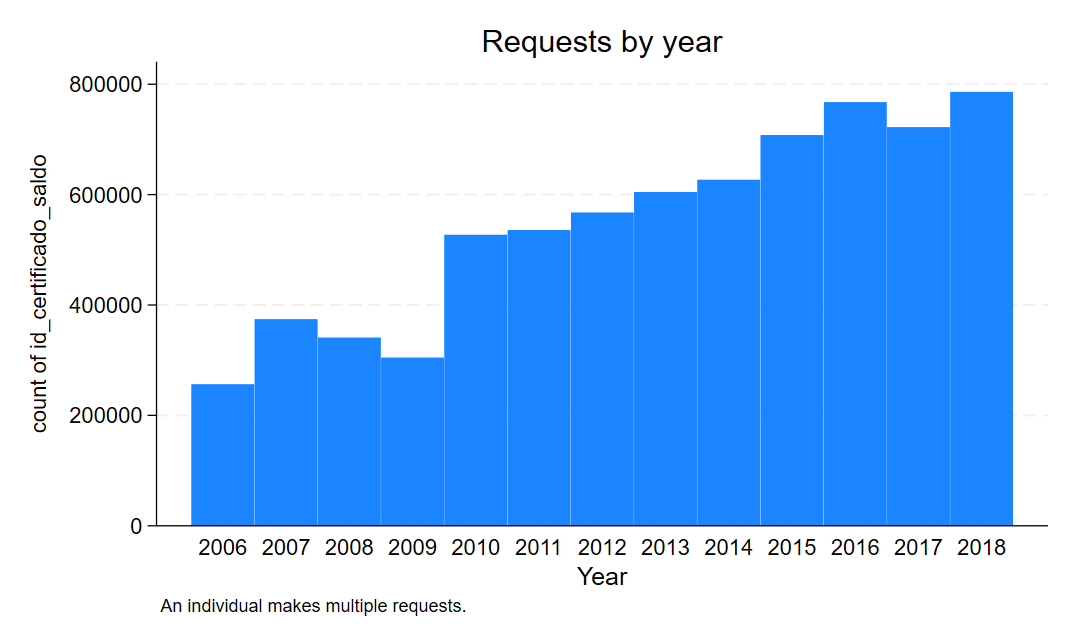
\includegraphics[scale=0.27]{figures/IE0_plot0.png}
\end{tabular}
\end{figure}


Figure \ref{fig:ie0_1} shows the amount of savings of individuals in the sample. Where 1UF is around 40 USD. The distribution is truncated at the 99th percentile of savings. 


\begin{figure}[H]
\caption{}
\label{fig:ie0_1}
\centering{}%
\begin{tabular}{cc}
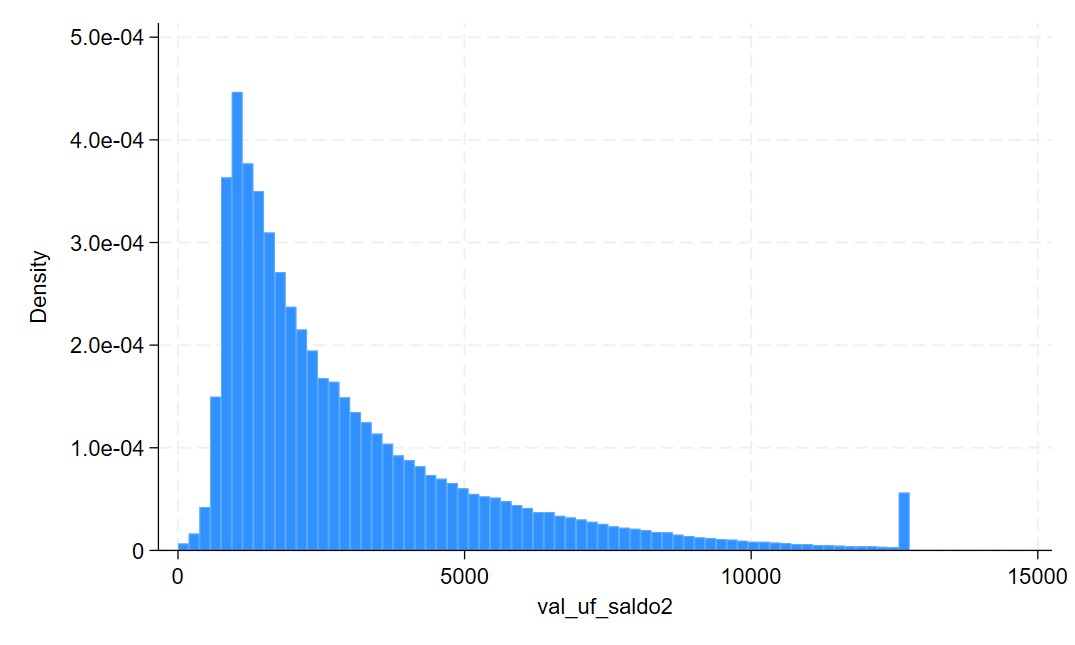
\includegraphics[scale=0.27]{figures/IE0_plot1.png} 
\end{tabular}
\end{figure}



Figure \ref{fig:ie0_2} shows the number of requests for each type of financial product in absolute terms and then their respective shares. The changes are not particularly large, it seems like the share of each financial product is relatively stable over time.

NOTE: ANNUITIES WITH PW(GREEN) START FROM 0 IN 2006 HENCE PROBABLY THEY ARE A FINANCIAL INNOVATION. 

\begin{figure}[H]
\caption{}
 \label{fig:ie0_2and3}
\centering{}%
\begin{tabular}{cc}
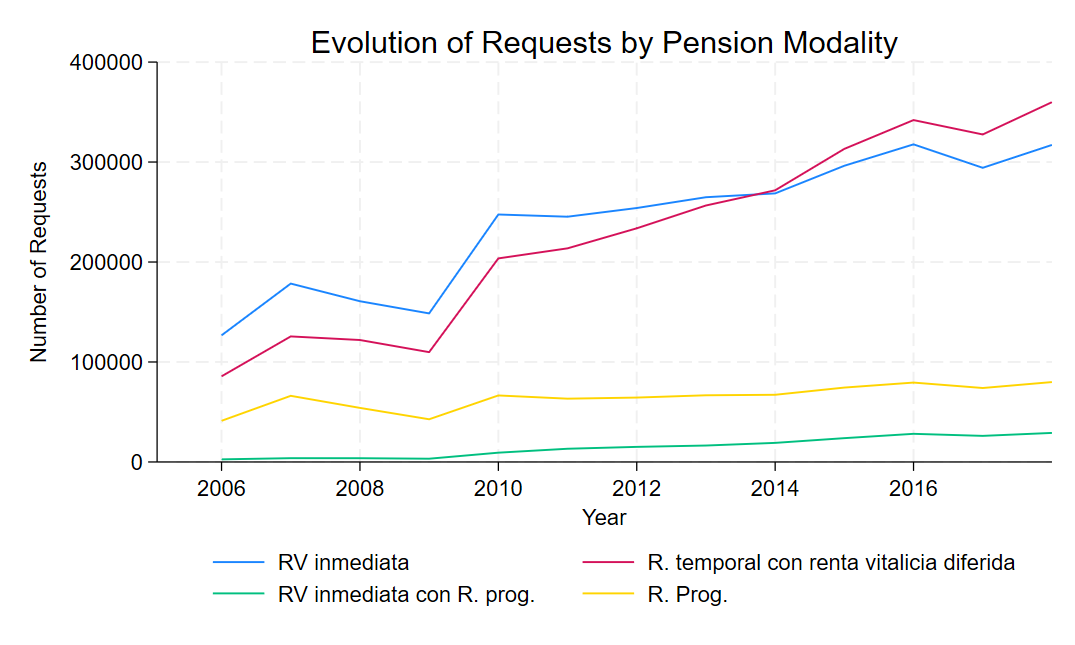
\includegraphics[scale=0.27]{figures/IE0_plot2.png} & 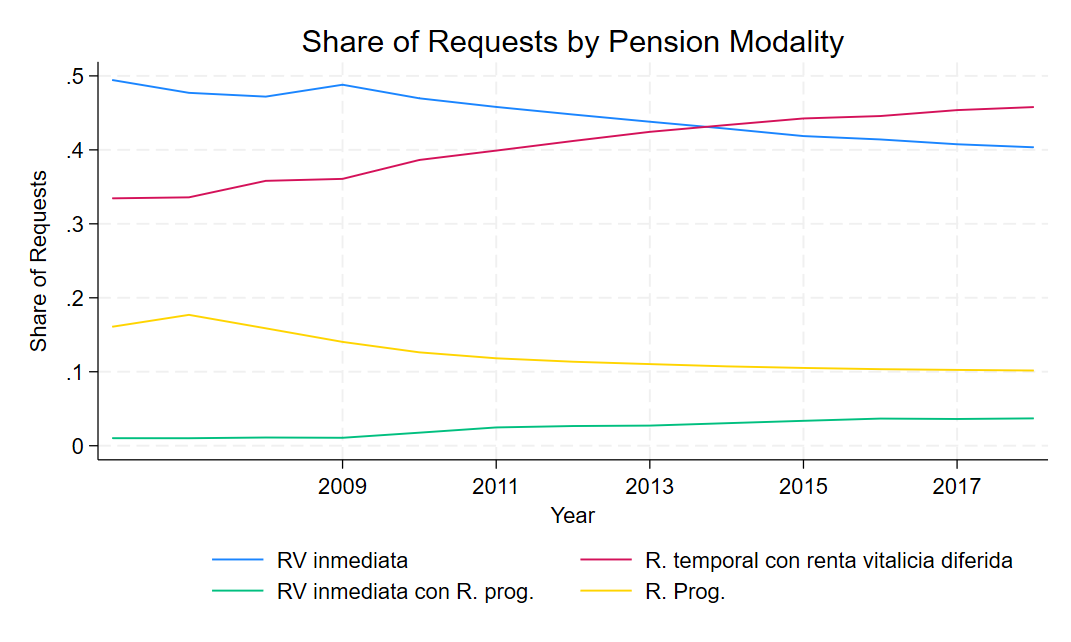
\includegraphics[scale=0.27]{figures/IE0_plot3.png}
\end{tabular}
\end{figure}


Figure \ref{fig:ie0_4} shows the shares for the whole sample as a function of savings. Richer individuals tend to buy more annuities with PW and less PW. This is explained by the fact that there is a minimum amount of savings required to buy an annuity and also could have to do with a higher life expectancy. 


\begin{figure}[H] 
\caption{}
\label{fig:ie0_4}
\centering{}%
\begin{tabular}{cc}
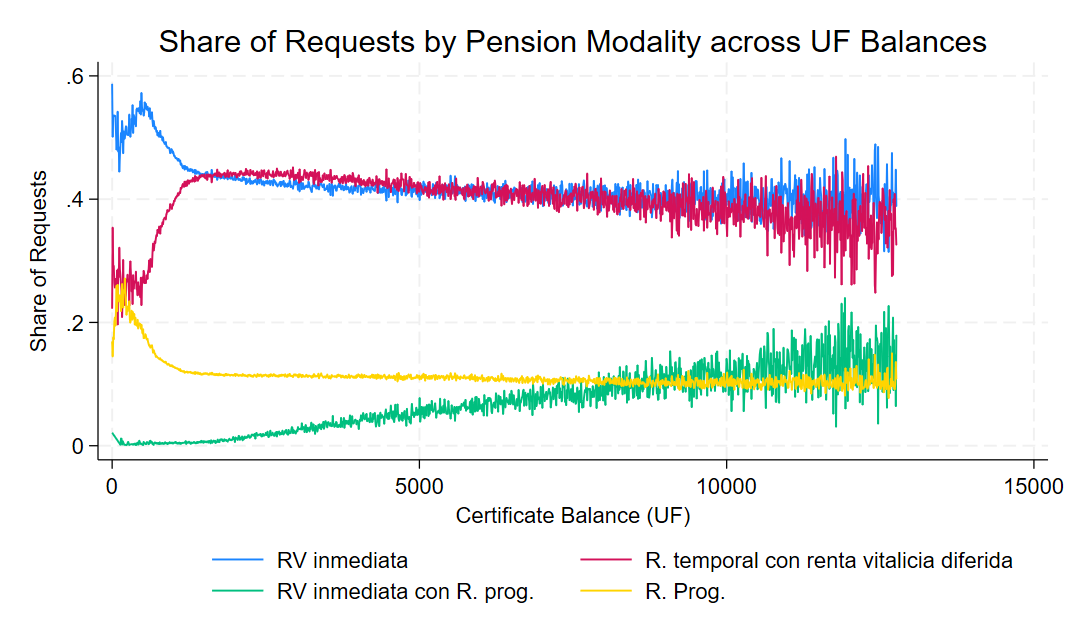
\includegraphics[scale=0.27]{figures/IE0_plot4.png}
\end{tabular}
\end{figure}

Figure \ref{fig:ie0_5} shows how many guaranteed months people buy. 
\begin{figure}[H] 
\caption{}
\label{fig:ie0_5}
\centering{}%
\begin{tabular}{cc}
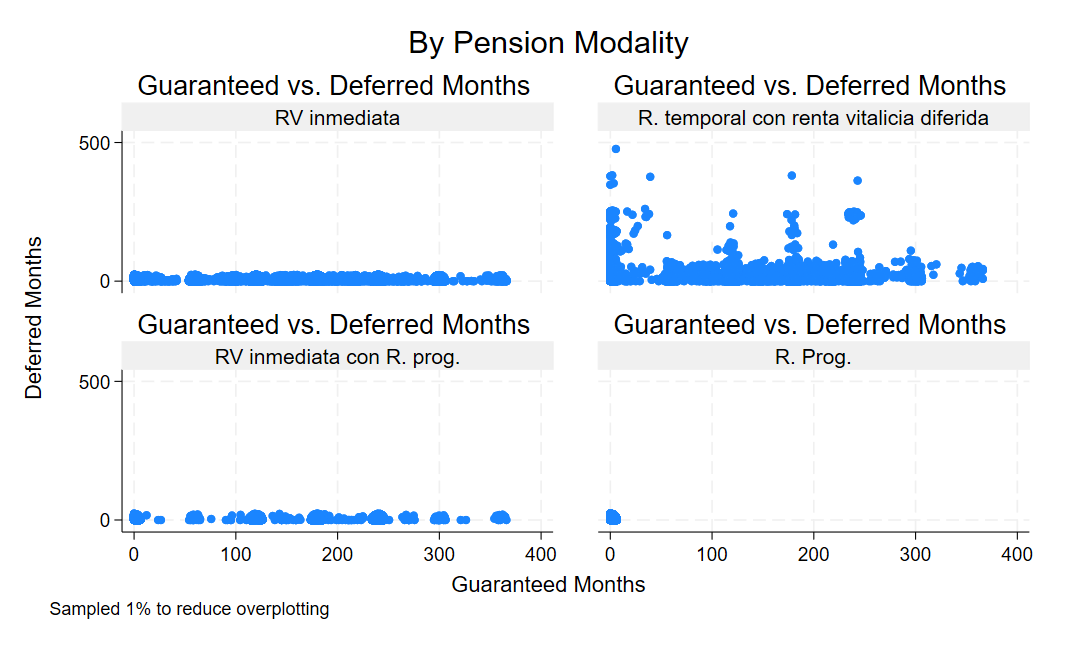
\includegraphics[scale=0.27]{figures/IE0_plot5.png}
\end{tabular}
\end{figure}

\section{IE 1}


Figure \ref{fig:ie1_1} the history of the credit rating for selected insurers.  
\begin{figure}[H]
\caption{}
 \label{fig:ie1_1}
\centering{}%
\begin{tabular}{cc}
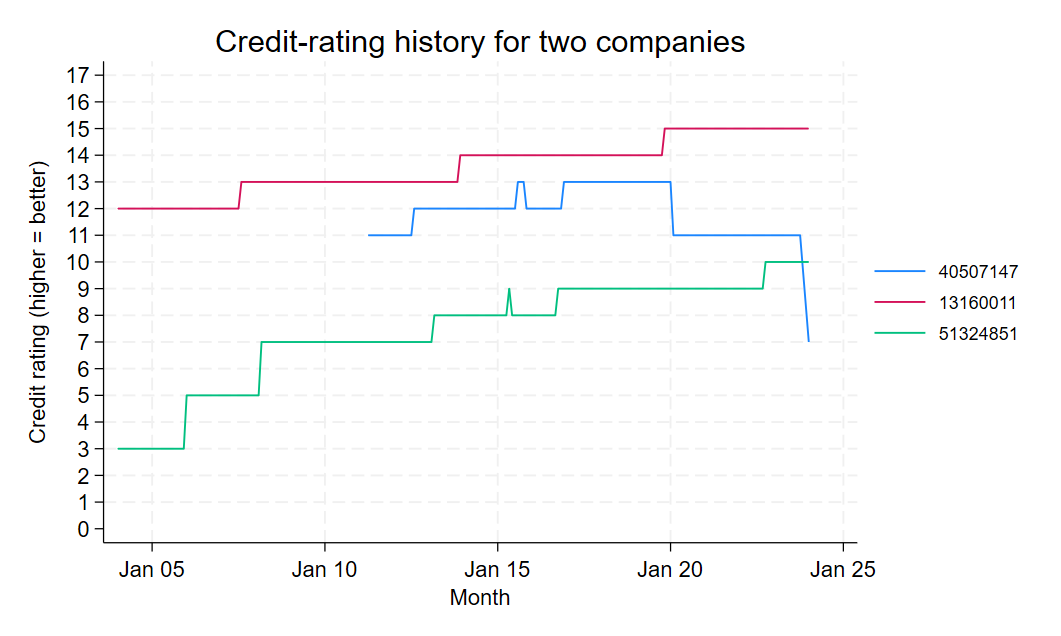
\includegraphics[scale=0.27]{figures/IE1_credit_history.png}
\end{tabular}
\end{figure}

Only 2\% of the offers constitute external offers, because individuals request offers from many financial products (make many requests), then receive many offers (one for each offering company) for each request, and then in case of requesting external offers they do it for only a subset of the initial offers. 

\section{IE1b}

This code just takes all the data of the offers (not only a sample) and creates .dta files where each of them contains a chunck of the data. Then filters the files to keep only the annuities and some years and finally joins all this filtered files into one big file with the offers. 
 

\section{IE 3}

Figure \ref{fig:ie3_0} shows the number of external offers that buyers request and figure \ref{fig:ie3_1} shows the distribution disaggregated by year. 

\begin{figure}[H]
\caption{}
\label{fig:ie3_0}
\centering{}%
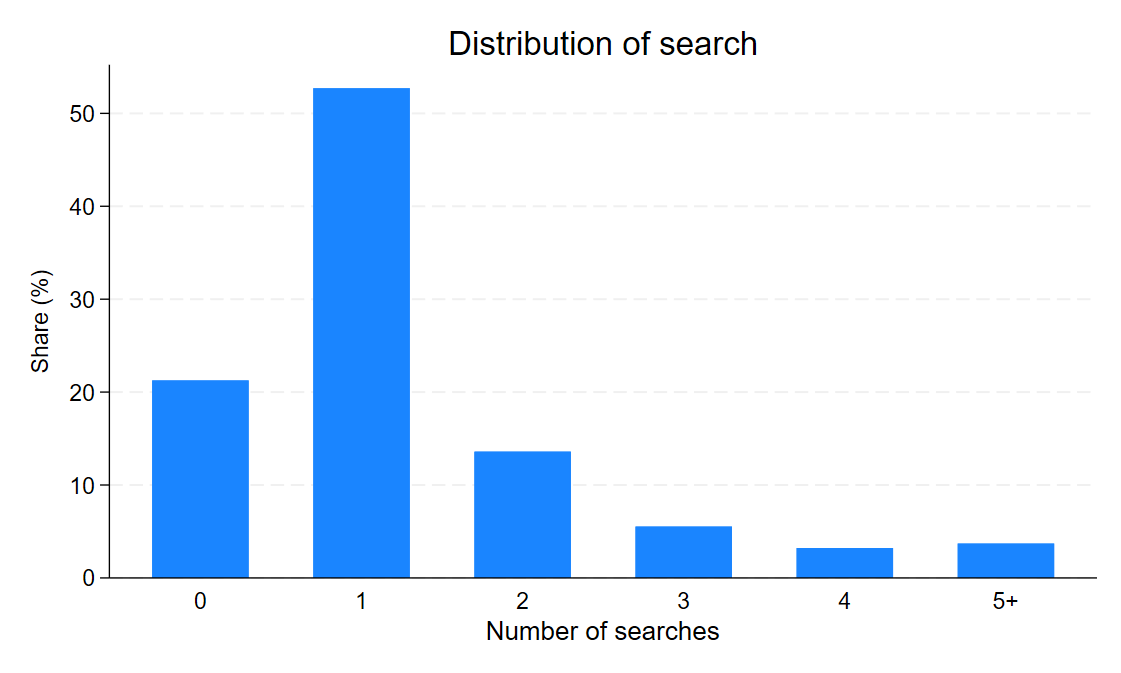
\includegraphics[scale=0.27]{figures/IE3_dist_external_offers.png}
\end{figure}


\begin{figure}[H]
\caption{}
\label{fig:ie3_1}
\centering{}%
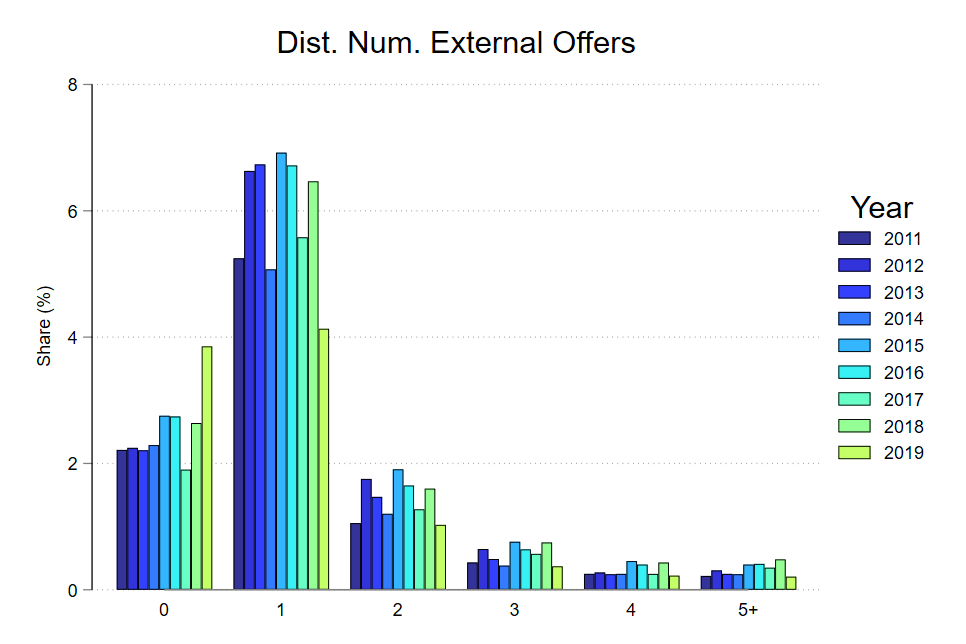
\includegraphics[scale=0.27]{figures/IE3_dist_external_offers_byyear.png}
\end{figure}


Figure \ref{fig:ie3_2} shows 

\begin{figure}[H]
\caption{}
 \label{fig:ie3_2}
\centering{}%
\begin{tabular}{cc}
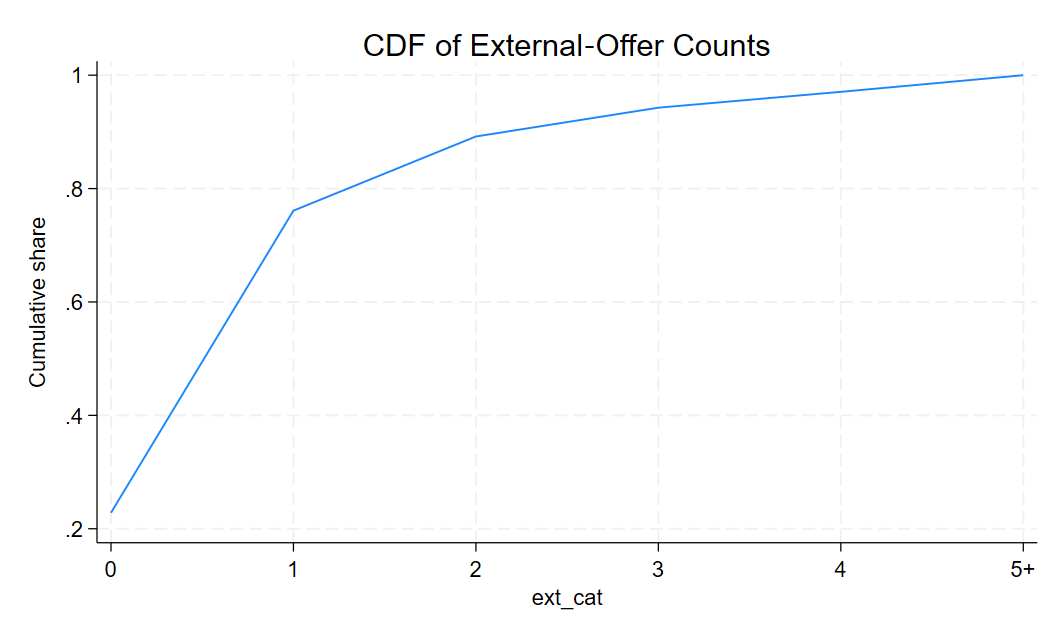
\includegraphics[scale=0.27]{figures/IE3_CDF_number_extoffers.png} &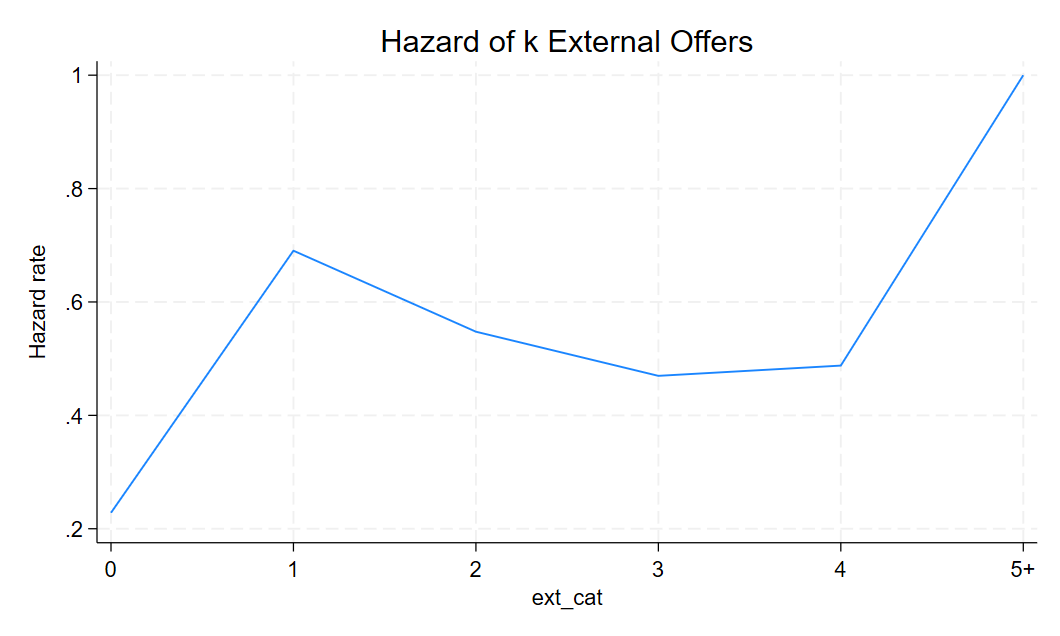
\includegraphics[scale=0.27]{figures/IE3_hazard_number_extoffers.png}
\end{tabular}
\end{figure}



Figure \ref{fig:ie3_3} shows the average number of searches for individuals grouped by their quintile of savings, which is a proxy of income. Specifically an increase of savings by a standard deviation is related to   0.30
 additional searches. 


\begin{figure}[H]
\caption{}
\label{fig:ie3_3}
\centering{}%
\begin{tabular}{cc}
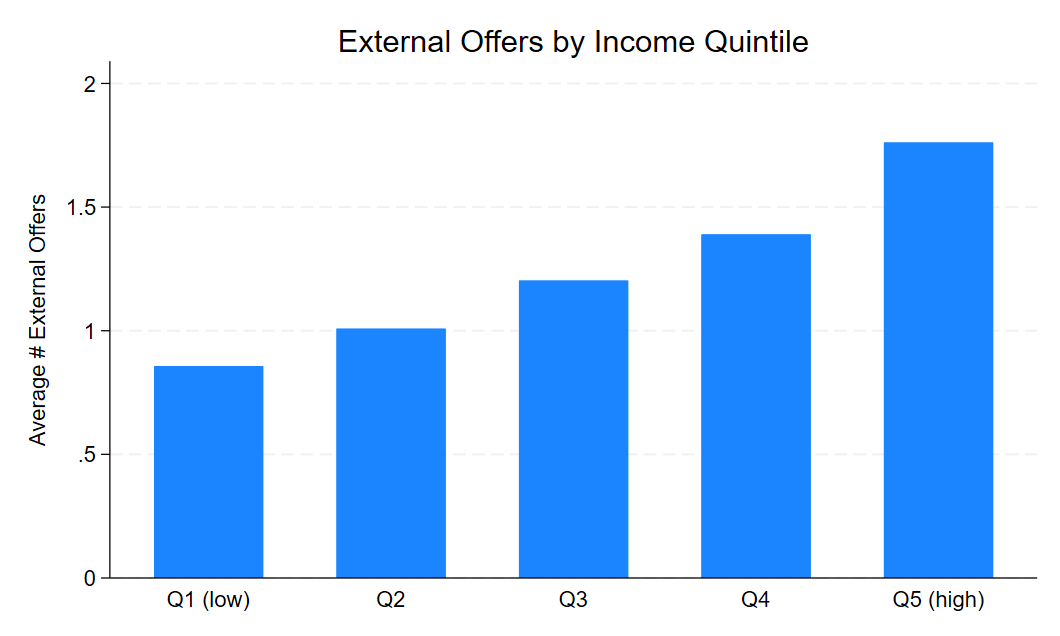
\includegraphics[scale=0.27]{figures/IE3_search_by_income_quintile.png}
\end{tabular}
\end{figure}

Figure \ref{fig:ie3_4} shows the CDF and hazard rate of searches grouped by savings quintile. 

\begin{figure}[H] 
\caption{}
\label{fig:ie3_4}
\centering{}%
\begin{tabular}{cc}
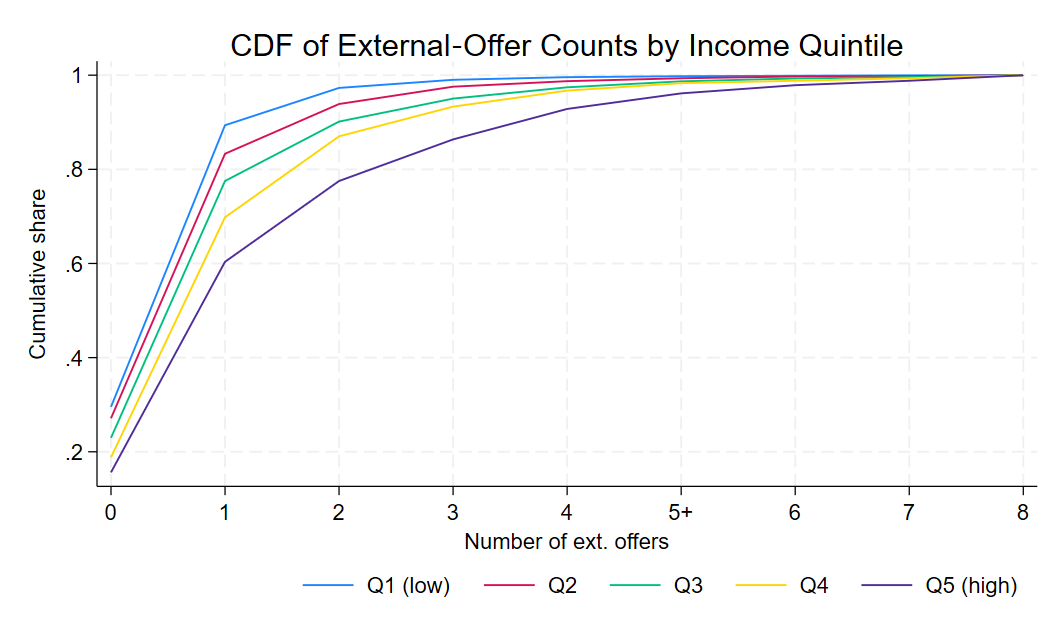
\includegraphics[scale=0.26]{figures/IE3_search_CDF_by_income_quintile.png} & 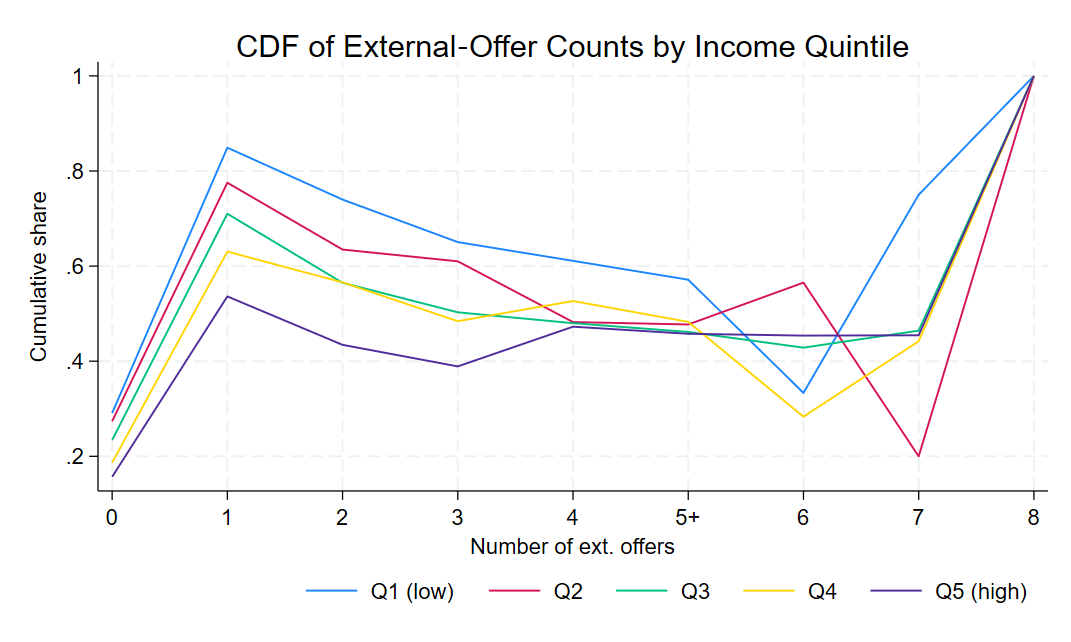
\includegraphics[scale=0.26]{figures/IE3_search_hazardrate_by_income_quintile.png}
\end{tabular}
\end{figure}


Figure \ref{fig:ie3_4b} shows the average number of searches for individuals grouped by their gender. Men do on average  -0.09
 more searches, which does not seem to be economically significant, although it is statistically significant.


\begin{figure}[H]
\caption{}
\label{fig:ie3_4b}
\centering{}%
\begin{tabular}{cc}
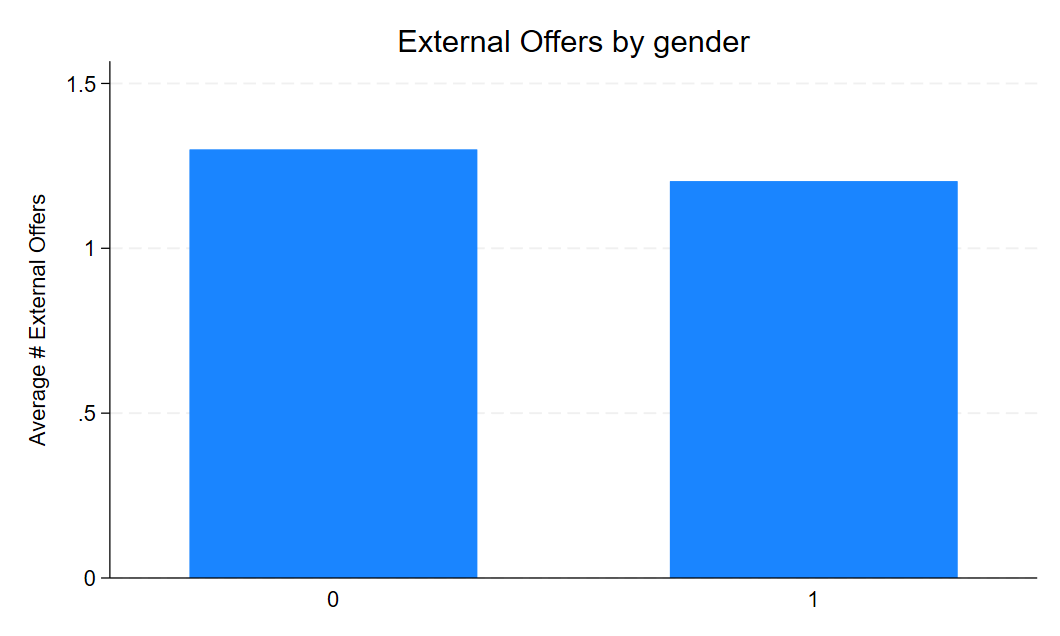
\includegraphics[scale=0.27]{figures/IE3_search_by_gender.png}
\end{tabular}
\end{figure}


\subsection{Dispersion in offers within group}

The insurers in the SCOMP platform observe the age, gender and savings \textcolor{red}{and same zip code?} of the individual. We want to see whether individuals with similar characteristics receive similar offers. 

Given the sparsity of the distribution of individuals it is difficult to find individuals with exactly the same characteristics. Hence we created three criteria to define a group: 
\begin{enumerate}
    \item Individuals within the 5-year age interval, same savings quintile and same gender who receive offers the same year by same firm. we call them group 1  
    \item Indivduals with the same age, gender and savings. who receive offers the same year by same firm. we call them group 2
    \item   Indivduals with the same age, gender and savings. we call them group 3
\end{enumerate}
where the first criteria is less sparse than the second, and the second is less sparse than the third. 
Note that using criteria 1 we could group a man of age 60 and savigs of 954 and and an individual of age 64 and savings of 1089, hence certain dispersion is expected. To reduce the role of savings on the offer dispersion we define the ratio as the savings didivded by the offer. 

Then we studied the dispersion of the offers within each group. 

The following table presents the summary statistics for dispersion variables. 
z\_offer is the percentual dispersion of the offers within groups formed by criteria 1, and then z\_offer2 and z\_offer3 for groups 2 and 3. Note that the variation is reduced once we define the groups using a finer criteria.

We exclude the external offers from the analysis since we expect them to be different from the internal offers. 


In row 3 we show the standard deviation of the offers using criteria 2. The average deviation is .51UF which is around 20USD. This dispersion could be justified by intermediaries, ZIP code, particular day, etc. 

\begin{table}[htbp]\centering
\def\sym#1{\ifmmode^{#1}\else\(^{#1}\)\fi}
\caption{Summary Statistics}
\begin{tabular}{l*{1}{ccccc}}
\hline\hline
            &\multicolumn{5}{c}{(1)}                                         \\
            &\multicolumn{5}{c}{}                                            \\
            &        mean&          sd&         min&         max&       count\\
\hline
z\_offer     &    .1991379&    .1166944&           0&    .8129947&      173923\\
z\_offer2    &    .1205333&    .0795119&           0&    .8659106&      171572\\
z\_offer3    &    .0638504&    .0510833&           0&    .3931563&       60530\\
sd\_offer3   &    .5127416&    .5968534&           0&    10.04091&       60530\\
\hline
\(N\)       &      173964&            &            &            &            \\
\hline\hline
\end{tabular}
\end{table}


Finally we run a regression of the offer on the group fixed effects. The coefficients are shown below. When using the finer group definition almost all the variation in offers is explained by the group fixed effects. 

\textbf{In terms of modeling, the previous findings suggest that we can assume that the insurers look at savings, gender and age and send offers based on these characteristics. }


\begin{tabular}{l*{3}{c}}
\hline\hline
            &      Group1&      Group2&      Group3\\
\hline
Val UF Pension&         .71&         .84&         .99\\
\hline\hline
\end{tabular}


\subsection{dispersion within group for external and internal offers. }

I used the 3 criteria to define groups presented previously and the within group standard deviation of the internal and external offers was not very different. I also run a regression of the offer on group fixed effects for the sample of internal and external offers and the R-squared was similar. 


\textcolor{red}{explain why I was expecting more diespersion for external offers.   and under which conditions this could be true. }
I had previously written "If there is revelation of information in the aftermarket then the R2 of the regression of the initial offers would be lower than for the external offers, since there would be information that firms are considering when bidding but which we do not have in our data. but is not the case"

\subsection{Others}

\subsubsection{Dispersion of the choice set}
Figure \ref{fig:ie3_5} shows the distribution of standard deviations of the choice set of the consumers and the left panel shows the distribution of the range, both of them normalized by the mean of the offers each individual receives.  The table below shows the summary statistics of both variables. Offers have an average deviation from the mean of the offers that represenet a 1.7\% of the mean offer and the range represent a 6\% of the mean offer. Considering that this are the savings of their lifetime, this differences translate into considerable absolute differences.

\begin{figure}[H] 
\caption{}
\label{fig:ie3_5}
\centering{}%
\begin{tabular}{cc}
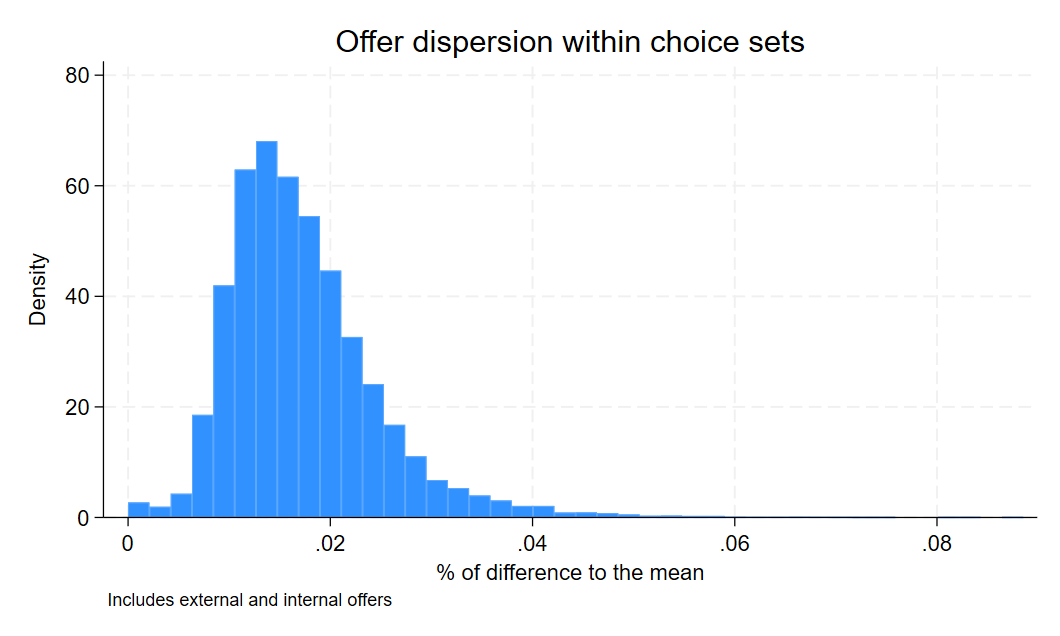
\includegraphics[scale=0.26]{figures/IE3_dispertion_choice_set.png} & 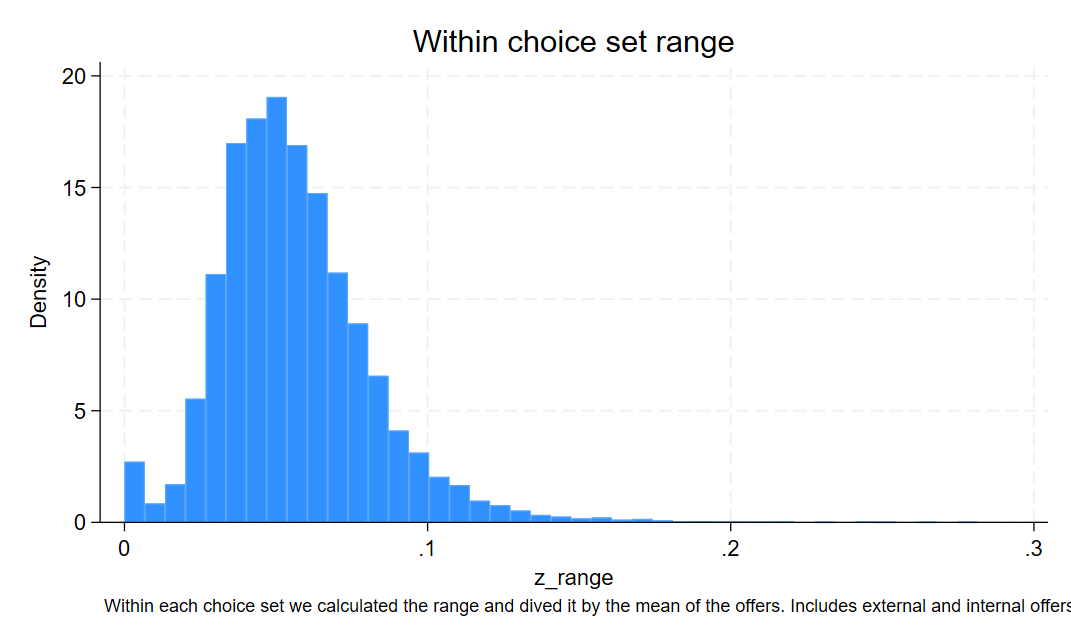
\includegraphics[scale=0.26]{figures/IE3_dispertion_choice_set_range.png}
\end{tabular}
\end{figure}


\begin{table}[htbp]\centering
\def\sym#1{\ifmmode^{#1}\else\(^{#1}\)\fi}
\caption{Summary Statistics}
\begin{tabular}{l*{1}{ccccc}}
\hline\hline
            &\multicolumn{5}{c}{(1)}                                         \\
            &\multicolumn{5}{c}{}                                            \\
            &        mean&          sd&         min&         max&       count\\
\hline
diff\_pct    &    .0176062&    .0072376&           0&    .0909576&      253280\\
z\_range     &    .0602848&    .0249717&           0&     .281407&      253468\\
\hline
\(N\)       &      253468&            &            &            &            \\
\hline\hline
\end{tabular}
\end{table}



\subsubsection{Improvement when asking for external offers}

The table below shows the improvement with respect to the initial offer made by the same company when asking for an external offer. The first row shows summary statistics for the absolute improvement, with a mean of .24 UF which is around 10 USD. The second row shows the improvement in percentage terms. The third column calculates the present value of the improvement, using the assumption that the individual lives 20 years and the monthly interest rate is 0.3\% which has been the average rate of return of the pension funds in the last 20 years \footnote{\href{https://bigdatauls.userena.cl/dashboards/rentabilidad-fondo-de-pensiones/}{source} note that the rate of return is in real terms because all the flows are in UF.}. Finally, to understand the dimension we take the previously calculated present value and divide it by the wage of the last month of the individual, on average the improvement in the offer corresponds to the salary of almost 4 months of work.  

\begin{table}[htbp]\centering
\def\sym#1{\ifmmode^{#1}\else\(^{#1}\)\fi}
\caption{Improvement when searching}
\begin{tabular}{l*{1}{ccccc}}
\hline\hline
            &\multicolumn{5}{c}{(1)}                                         \\
            &\multicolumn{5}{c}{}                                            \\
            &        mean&          sd&         min&         max&       count\\
\hline
improvement\_abs&    .2429171&    .2865748&   -.6700001&    9.050003&       19142\\
improvement\_pct&    1.763955&    1.303467&   -10.48513&    15.43956&       19142\\
improvement\_PV20&    41.51639&    48.97782&   -114.5081&    1546.714&       19142\\
improvement\_wage&    3.922188&    35.43327&   -2.413689&    2802.884&       19038\\
\hline
\(N\)       &       19142&            &            &            &            \\
\hline\hline
\end{tabular}
\end{table}


\begin{figure}[H]
\caption{}
\label{fig:aux}
\centering{}%
\begin{tabular}{cc}
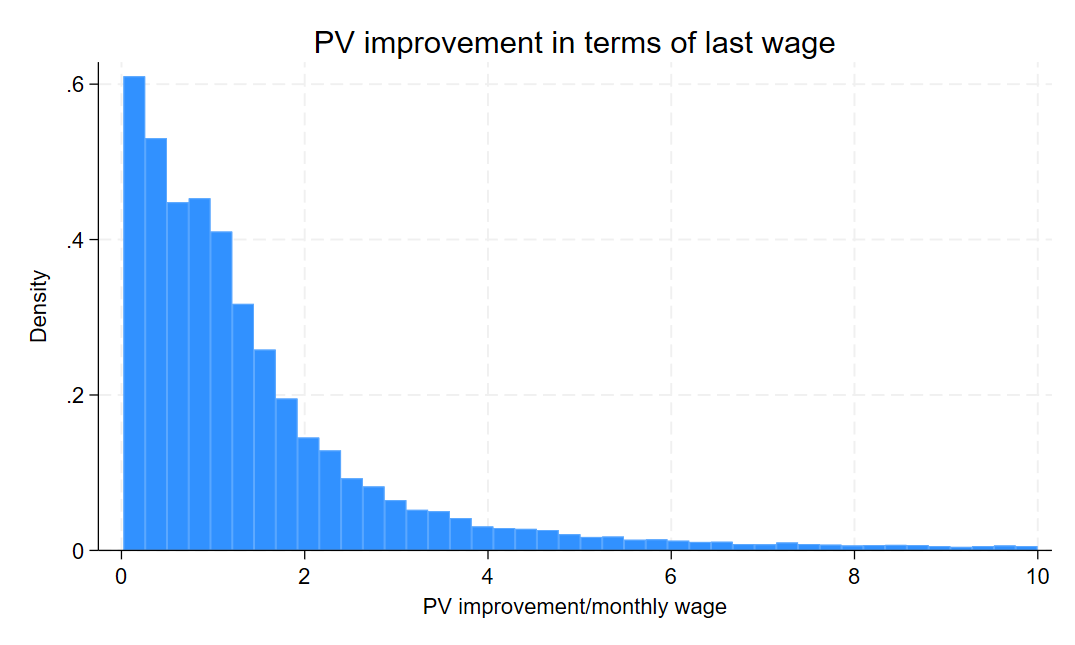
\includegraphics[scale=0.3]{figures/IE3_offer_improvement_histogram.png}
\end{tabular}
\end{figure}



Figure \ref{fig:aux} shows the summary statistics of the distribution of the different measures of improvement desaggregated by gender. On average men get a higher absolute improvement, but since they also have higher initial offers (due to their higher savings) women get a higher improvement in percentage terms.
\begin{figure}[H]
\caption{}
\label{fig:aux}
\centering{}%
\begin{tabular}{cc}
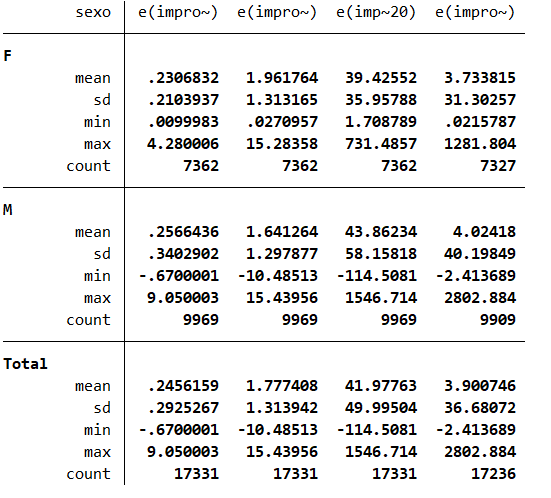
\includegraphics[scale=0.7]{Tables/IE3_offer_improvement_bygender.png}
\end{tabular}
\end{figure}



Figure \ref{fig:aux2} shows the summary statistics of the distribution of the different measures of improvement desaggregated by income quintile. Higher quintiles get bigger improvements (col1) but in terms of the percentual improvement there does not seem to be a clear pattern (col2). Finally almost all groups get an increase which in PV corresoponds to around 5 months of work, with the exception of the first quintile, were buyers get only 2 months of work on average. 
\begin{figure}[H]
\caption{}
\label{fig:aux2}
\centering{}%
\begin{tabular}{cc}
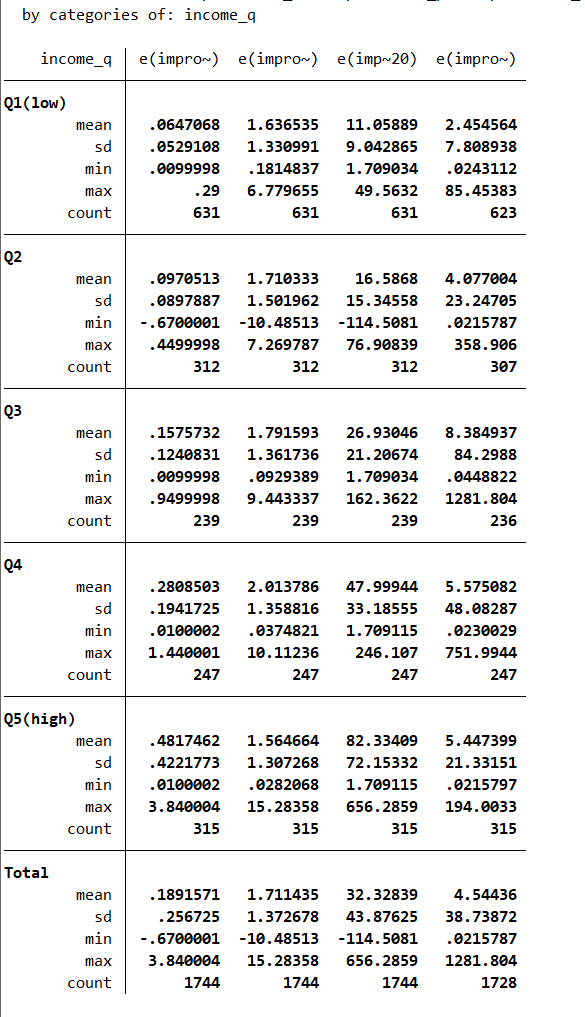
\includegraphics[scale=0.7]{Tables/IE3_offer_improvement_byincomequintile.png}
\end{tabular}
\end{figure}


\subsubsection{Improvement when asking for external offers wrt to highest offer}

The table below shows the improvement with respect to the highest initial offer when asking for an external offer. Sometimes the external offer is higher and sometimes lower than the higher internal offer but on average they are the same (the highest initial offer is only .03\% higher than the external offer), but with considerable dispersion, see figure \ref{fig:ie3_6}. 


\begin{table}[htbp]\centering
\def\sym#1{\ifmmode^{#1}\else\(^{#1}\)\fi}
\caption{External offer vs. highest initial offer}
\begin{tabular}{l*{1}{ccccc}}
\hline\hline
            &\multicolumn{5}{c}{(1)}                                         \\
            &\multicolumn{5}{c}{}                                            \\
            &        mean&          sd&         min&         max&       count\\
\hline
diff        &   -.0268622&    .4096033&      -16.45&    2.610001&      179605\\
diff\_pct    &    .0000994&    1.673789&   -13.11523&    12.01414&      179605\\
\hline
\(N\)       &      179605&            &            &            &            \\
\hline\hline
\multicolumn{6}{l}{\footnotesize hola}\\
\end{tabular}
\end{table}



\begin{figure}[H]
\caption{}
\label{fig:ie3_6}
\centering{}%
\begin{tabular}{cc}
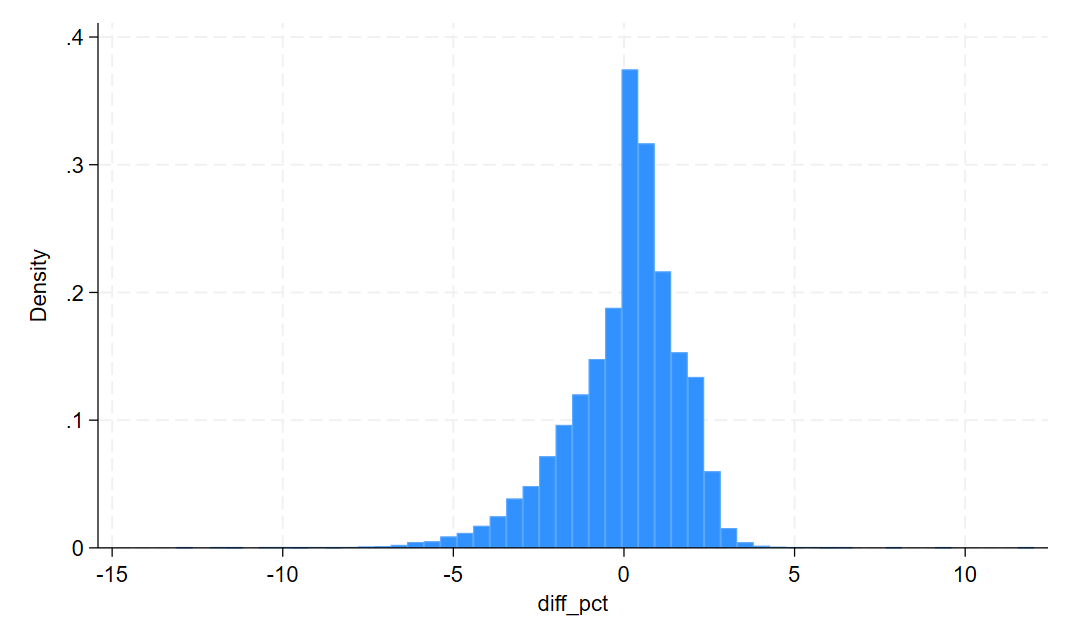
\includegraphics[scale=0.27]{figures/IE3_offer_change_max_internal.png}
\end{tabular}
\end{figure}


\subsubsection{Number of initial offers}


Almost all the insurers bid in the first round. , see table below.

\begin{table}[htbp]\centering
\def\sym#1{\ifmmode^{#1}\else\(^{#1}\)\fi}
\caption{Dist. of number of initial offers}
\begin{tabular}{l*{1}{ccccc}}
\hline\hline
            &\multicolumn{5}{c}{(1)}                                         \\
            &\multicolumn{5}{c}{}                                            \\
            &        mean&          sd&         min&         max&       count\\
\hline
internal\_offers&    10.52688&    3.189377&           1&          31&       21929\\
\hline
\(N\)       &       21929&            &            &            &            \\
\hline\hline
\end{tabular}
\end{table}


\subsubsection{Discrete choice determinants}

The share of buyers who end up buying an annuity that is not the highest offer is:  0.462
. Moreover when they do not buy the highest offer they choose offers which are significantly lower. Figure \ref{fig:ie3_7} shows the distribution of the highest offer minus the chosen offer (foregone amount) as a share of the accepted offer in percentage terms. 

And the table below shows in the first row the average foregone percentage among the buyers who did not choose the highest offer. 1.5\% might not seem like a lot, but if we assume that the buyer has 20 years of life left and we use a .03\% monthly interest rate  \footnote{previously explained why is sensible} it means they are foregoing almost 20 UF in present value terms, which when divided by the last monthly salary of the individual is around 1.6 months of salary. 


\begin{figure}[H]
\caption{}
\label{fig:ie3_7}
\centering{}%
\begin{tabular}{cc}
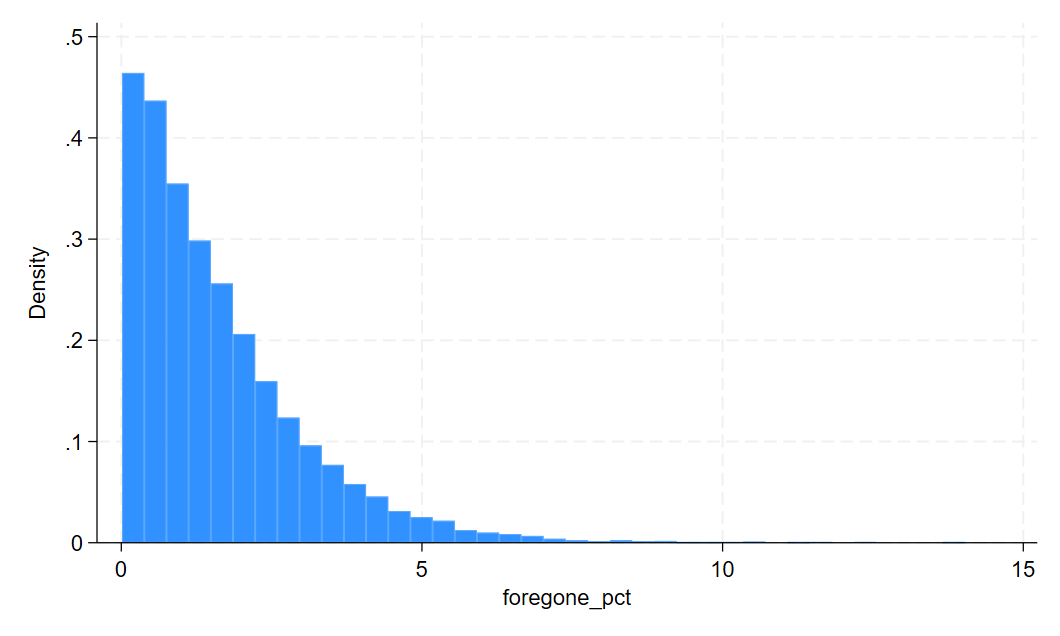
\includegraphics[scale=0.27]{figures/IE3_foregone_hist.png}
\end{tabular}
\end{figure}

\begin{table}[htbp]\centering
\def\sym#1{\ifmmode^{#1}\else\(^{#1}\)\fi}
\caption{Foregone pension}
\begin{tabular}{l*{1}{ccccc}}
\hline\hline
            &\multicolumn{5}{c}{(1)}                                         \\
            &\multicolumn{5}{c}{}                                            \\
            &        mean&          sd&         min&         max&       count\\
\hline
foregone\_pct&    1.532654&    1.377626&    .0132041&      14.029&      118922\\
foregonePV20&    19.19899&     58.0713&           0&     2811.43&      253468\\
foregone\_wage&    1.552708&    16.61985&           0&    1452.715&      252179\\
\hline
\(N\)       &      253468&            &            &            &            \\
\hline\hline
\end{tabular}
\end{table}


One possibility is that buyers perceive insurers as differentiated,for example in conversations with a financial advisor they mentioned the importance of risk rating of the insurer\footnote{See conversation with Claudia Ayala (9 jul 25), where she says: \textit{ la clasificación en una Compañía de Seguros es muy importante porque demuestra la espalda financiera de cada una de ellas, como se encuentra en posición al resto, sucursales, spot venta, es decir un servicio completo, EN EL FONDO QUE NOS ENTREGA ... UNA TRANQUILIDAD EN EL PAGO DE PENSIONES FUTURAS}}, the customer service or the brand appeal of the company. 

\begin{table}[htbp]\centering
\def\sym#1{\ifmmode^{#1}\else\(^{#1}\)\fi}
\caption{Acceptance (clogit) Results}
\begin{tabular}{l*{1}{c}}
\hline\hline
                    &\multicolumn{1}{c}{(1)}         \\
\hline
accepted2           &                     \\
Standarizd amount   &      13.956\sym{***}\\
                    &     (0.144)         \\
[1em]
Standarized risk score&       1.253\sym{***}\\
                    &     (0.044)         \\
\hline
Obs.                &     228,287         \\
\hline\hline
\multicolumn{2}{l}{\footnotesize Standard errors in parentheses}\\
\multicolumn{2}{l}{\footnotesize Variables are standarized at the choice set level}\\
\multicolumn{2}{l}{\footnotesize \sym{*} \(p<0.10\), \sym{**} \(p<0.05\), \sym{***} \(p<0.01\)}\\
\end{tabular}
\end{table}


To assess the possibility that buyers perceive insurers as differentiated, we run a conditional logit regression on the choice set of the buyers, and as expected we observe that although the primary determinant of the choice is the amount of the offer, the risk rating of the insurer does affect the choice. 

\subsubsection{Death and external offers}
When bargaining for an external offer one can always disclose personal health information. Possibilities 
\begin{itemize}
    \item Sick individuals are more likely to ask for external offers
    
    The first table below shows the tabulation of individuals who die in our data (rows) with  a dummy for whether they asked for external offers(cols). Then the second table shows the share of individuals who negotiate an external offer by their current status. Individuals who already died also are less likely to ask for external offers. 

    \begin{table}[htbp]\centering
\def\sym#1{\ifmmode^{#1}\else\(^{#1}\)\fi}
\caption{Cross-tabulation of Death Status and External Status}
\begin{tabular}{l*{3}{c}}
\hline\hline
            &           0&           1&       Total\\
            &           b&           b&           b\\
\hline
0           &        3453&       11729&       15182\\
1           &         309&         996&        1305\\
Total       &        3762&       12725&       16487\\
\hline\hline
\end{tabular}
\end{table}

    Then when running a logit model of the probability of asking for an external offer on whether the buyer is dead and year fixed effect, we find that already dead individuals asked for fewer external offers. 

    \textcolor{red}{ to icnrease the sample size I can also use all the other annuities}



\begin{table}[htbp]\centering
\def\sym#1{\ifmmode^{#1}\else\(^{#1}\)\fi}
\caption{}
\begin{tabular}{l*{1}{ccccc}}
\hline\hline
            &\multicolumn{5}{c}{(1)}                                         \\
            &\multicolumn{5}{c}{}                                            \\
            &        mean&          sd&         min&         max&       count\\
\hline
has\_ex\_alive&    .7725596&    .4191931&           0&           1&       15182\\
has\_ex\_dead &    .7632184&    .4252701&           0&           1&        1305\\
\hline
\(N\)       &       16487&            &            &            &            \\
\hline\hline
\end{tabular}
\end{table}


\begin{table}[htbp]\centering
\def\sym#1{\ifmmode^{#1}\else\(^{#1}\)\fi}
\caption{Acceptance (clogit) Results}
\begin{tabular}{l*{1}{c}}
\hline\hline
                    &\multicolumn{1}{c}{(1)}         \\
\hline
has\_external        &                     \\
dead                &      -0.033\sym{*}  \\
                    &     (0.019)         \\
[1em]
val\_uf\_prima        &       0.000\sym{***}\\
                    &     (0.000)         \\
\hline
Obs.                &     253,468         \\
\hline\hline
\multicolumn{2}{l}{\footnotesize Standard errors in parentheses}\\
\multicolumn{2}{l}{\footnotesize Includes year fixed effects}\\
\multicolumn{2}{l}{\footnotesize \sym{*} \(p<0.10\), \sym{**} \(p<0.05\), \sym{***} \(p<0.01\)}\\
\end{tabular}
\end{table}

\newpage
    \item Sick individuals get higher increases when bargaining 
    
    One could think that less healthy individuals when bargaining with firms can reveal their lower life expectancy and hence get higher increases in the offers. This appears not to be the case, conditional on bargaining dead and alive individuals get similar increases in the offers. 

    To explore this possibility we first run a regression of the percentual improvement of the initial offer when the buyer approaches the insurer to bargain, we observe that individuals who already died in our data actually get lower increases in the offers. 

    Then we run a regression of the improvment on the dead dummy and year fixed effects to account for possible trends in negotiation rates in our data. The coefficient is negative which suggests that actually healthier individuals get higher increases in the offers.

    \begin{table}[htbp]\centering
\def\sym#1{\ifmmode^{#1}\else\(^{#1}\)\fi}
\caption{T-test: Improvement Percentage by Death Status}
\begin{tabular}{l*{1}{cccccc}}
\hline\hline
            & Mean Dead=0& Mean Dead=1&  Difference         &  Std. Error& t-statistic&     p-value\\
\hline
improvement\_pct&       1.790&       1.614&       0.176\sym{***}&       0.039&       4.531&       0.000\\
\hline
\(N\)       &       17331&            &                     &            &            &            \\
\hline\hline
\multicolumn{7}{l}{\footnotesize *** p<0.01, ** p<0.05, * p<0.1}\\
\end{tabular}
\end{table}


    \begin{table}[htbp]\centering
\def\sym#1{\ifmmode^{#1}\else\(^{#1}\)\fi}
\caption{Effect of bad health on negotiation gains}
\begin{tabular}{l*{1}{c}}
\hline\hline
                    &\multicolumn{1}{c}{(1)}         \\
\hline
dead                &      -0.137\sym{***}\\
                    &     (0.035)         \\
\hline
Obs.                &      19,142         \\
\hline\hline
\multicolumn{2}{l}{\footnotesize Standard errors in parentheses}\\
\multicolumn{2}{l}{\footnotesize Includes year fixed effects}\\
\multicolumn{2}{l}{\footnotesize \sym{*} \(p<0.10\), \sym{**} \(p<0.05\), \sym{***} \(p<0.01\)}\\
\end{tabular}
\end{table}



\end{itemize}


\subsection{Supply side}

\subsubsection{Market share of insurers}
Figures \ref{fig:ie3_9}, \ref{fig:ie3_10} and \ref{fig:ie3_11} show the market share of the insurers among different groups of the population. 
For example in figure \ref{fig:ie3_9} we see that the market share of insurer 827... is higher among older buyers whereas insurer 201... has just the opposite pattern. 
In figure \ref{fig:ie3_10} we see that insurer 997... sells mostly to rich consumers whereas insurer 585... sells mostly to poor consumers. 


\begin{figure}[H]
\caption{}
\label{fig:ie3_9}
\centering{}%
\begin{tabular}{cc}
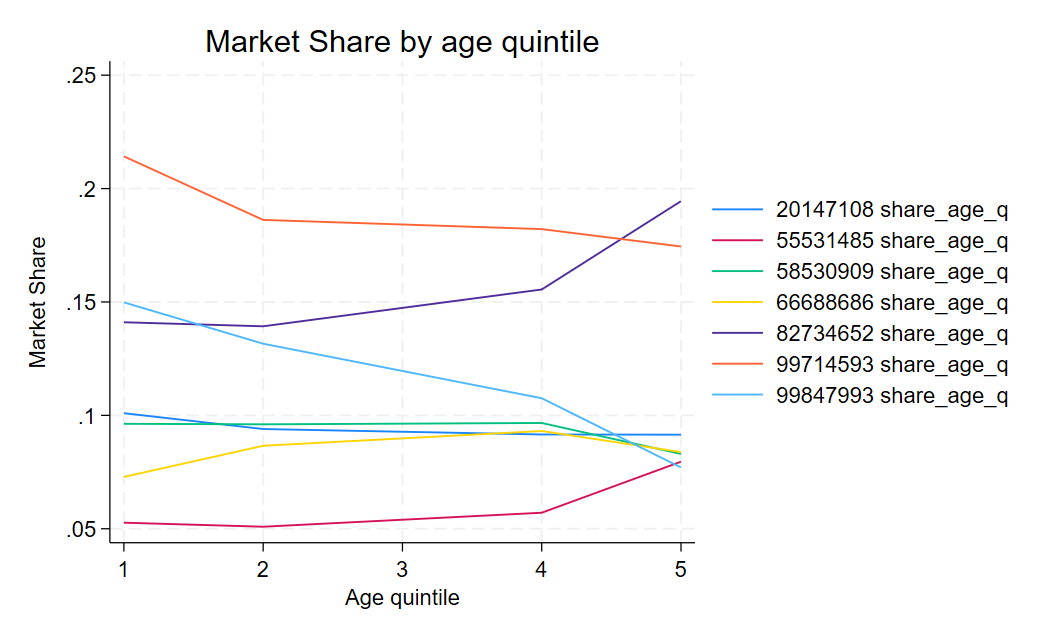
\includegraphics[scale=0.27]{figures/IE3_supply_age_quintile.png}
\end{tabular}
\end{figure}

\begin{figure}[H]
\caption{}
\label{fig:ie3_10}
\centering{}%
\begin{tabular}{cc}
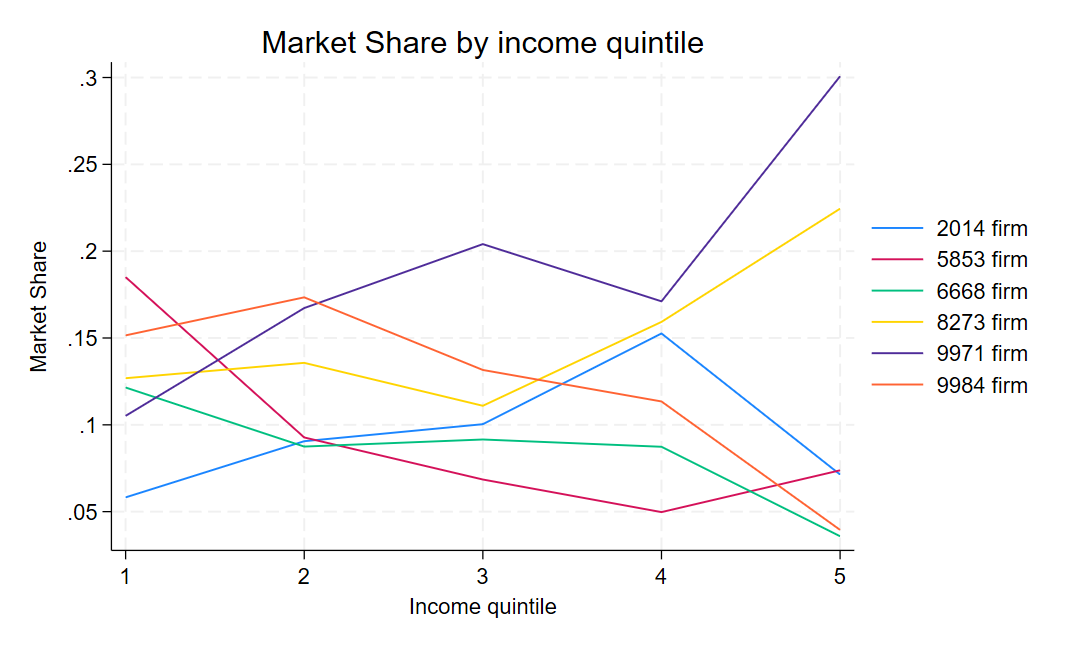
\includegraphics[scale=0.27]{figures/IE3_supply_income_quintile.png}
\end{tabular}
\end{figure}


\begin{figure}[H] 
\caption{}
\label{fig:ie3_11}
\centering{}%
\begin{tabular}{cc}
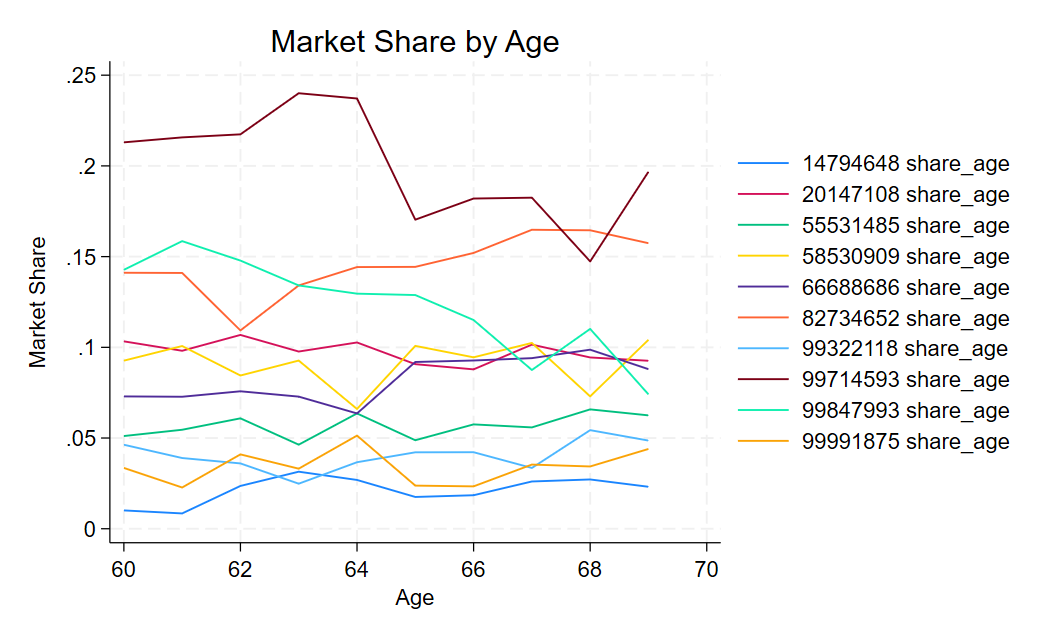
\includegraphics[scale=0.24]{figures/IE3_supply_age.png} &
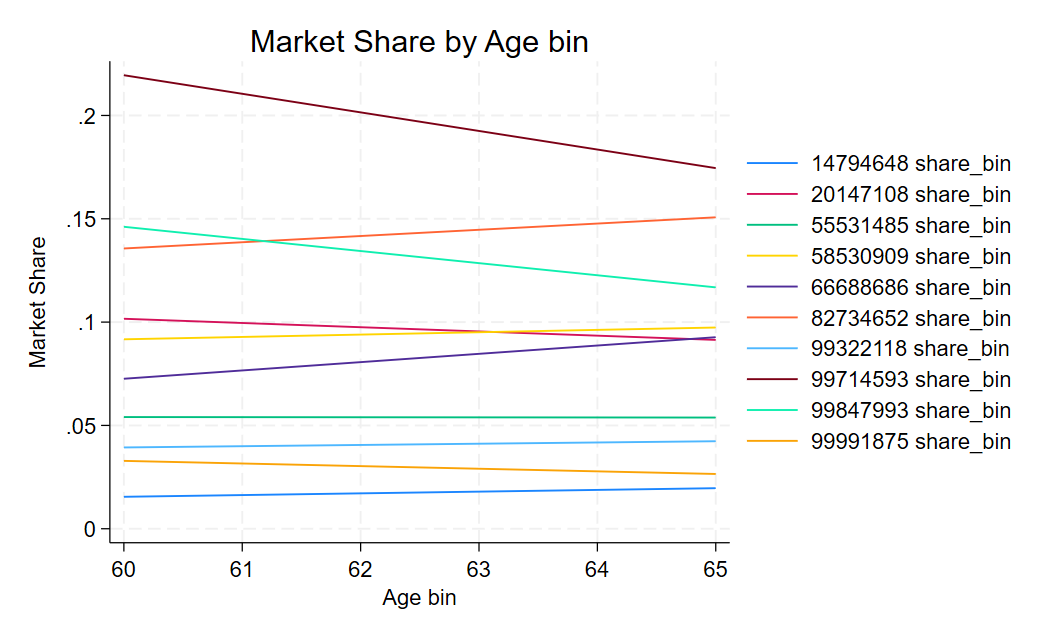
\includegraphics[scale=0.24]{figures/IE3_supply_agebin.png}
\end{tabular}
\end{figure}


\subsubsection{Probability of offer}
Figures \ref{fig:ie3_12}, \ref{fig:ie3_13} and \ref{fig:ie3_14} show the probability an insurer sends an offer to each of the different segments of buyers. 




For example in figure \ref{fig:ie3_12} we see that the insurer 1479... almost always makes an offer, whereas insurer 997... targets the income quintiles 2,3 and 4, and the probability of making an offer to quintile 1 is essentially zero. 

There does not appear to be so much targeting by age, see figure \ref{fig:ie3_13} and \ref{fig:ie3_14} where the lines are more horizontal than in the case of income. But what is striking is that there is high heterogeneity in the probability of making an offer at all, in our sample firm 345... makes an offer in around 20\% of the cases, whereas firm 1479... makes an offer in almost all the cases.
One possibility is that the previous pattern is caused by firms not being present all the years in our data, but when they are active they always make an offer. To check this we replicate figure \ref{fig:ie3_14} but by year for the years 2012-2015. We see that this pattern holds for the individual years. 


\textcolor{red}{THE BIG QUESTION IS WHY DO SOME FIRMS MAKE OFFERS ONLY TO SOME SEGMENTS OF THE POPULATION? AND EXACTLY TO WHAT SEGMENTS? IT COULD BE DEMAND DRIVEN (SOME SEGMENTS PREFER INSURER A, HENCE INSURER B DOES NOT EVEN TRY TO SELL THEM) OR SUPPLY DRIVEN. BUT THERE SEEMS TO BE SOMETHING INTERESTING HERE.}


\begin{figure}[H]
\caption{}
\label{fig:ie3_12}
\centering{}%
\begin{tabular}{cc}
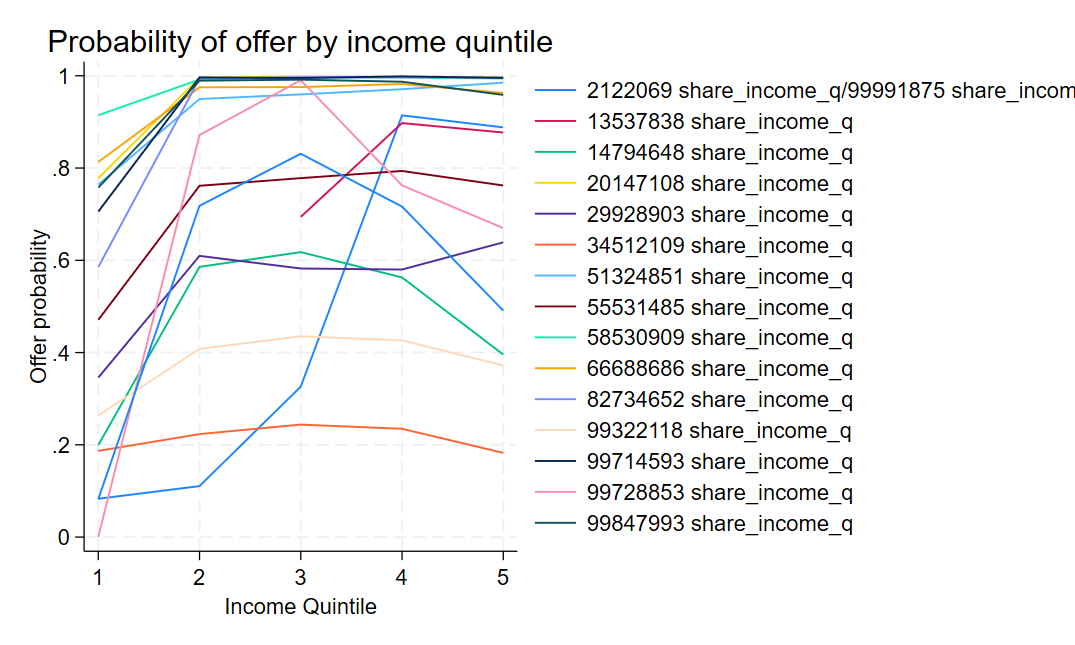
\includegraphics[scale=0.27]{figures/IE3_supply_offerprob_income_q.png}
\end{tabular}
\end{figure}


\begin{figure}[H]
\caption{}
\label{fig:ie3_13}
\centering{}%
\begin{tabular}{cc}
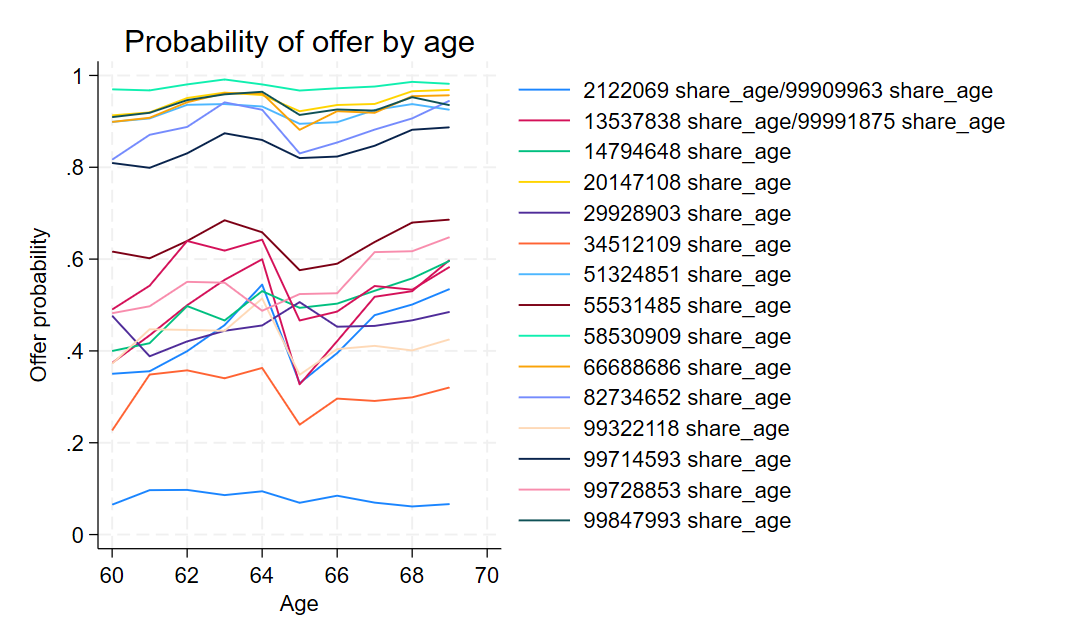
\includegraphics[scale=0.27]{figures/IE3_supply_offerprob_age.png}
\end{tabular}
\end{figure}


\begin{figure}[H] 
\caption{}
\label{fig:ie3_14}
\centering{}%
\begin{tabular}{cc}
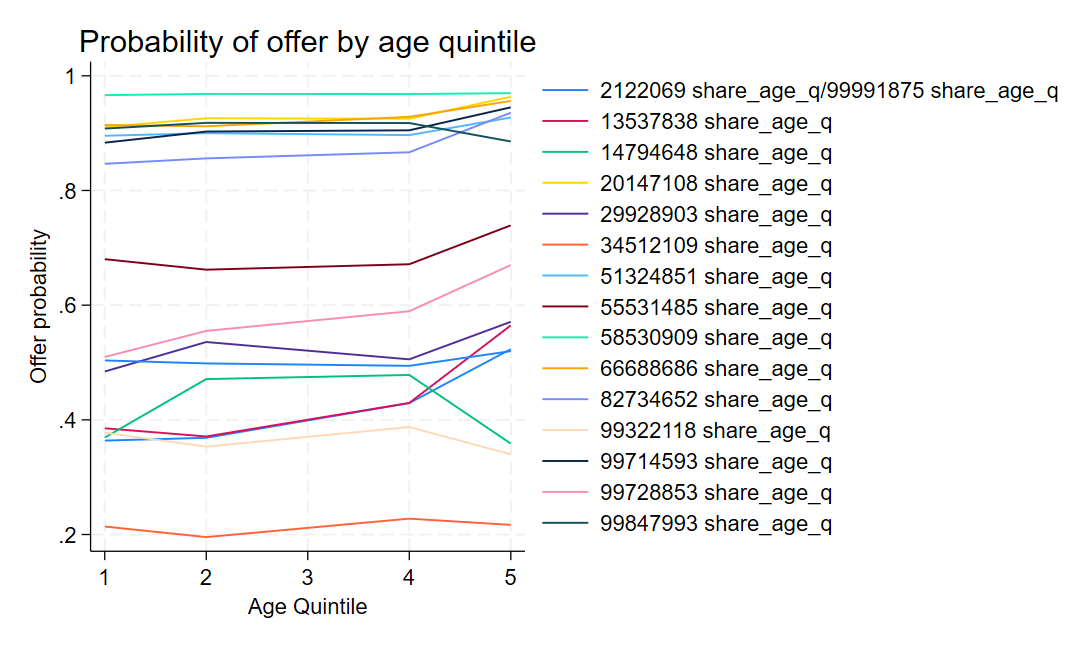
\includegraphics[scale=0.27]{figures/IE3_supply_offerprob_age_q.png}
\end{tabular}
\end{figure}




\begin{figure}[H] 
\caption{}
\label{fig:ie3_15}
\centering{}%
\begin{tabular}{cc}
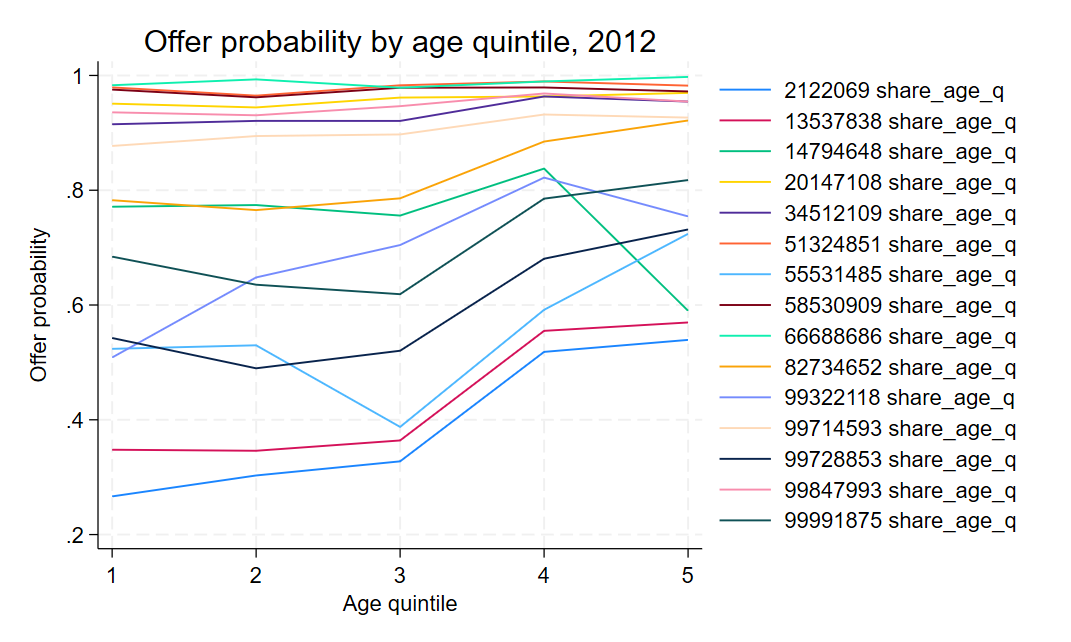
\includegraphics[scale=0.27]{figures/IE3_supply_offerprob_age_q_2012.png} &
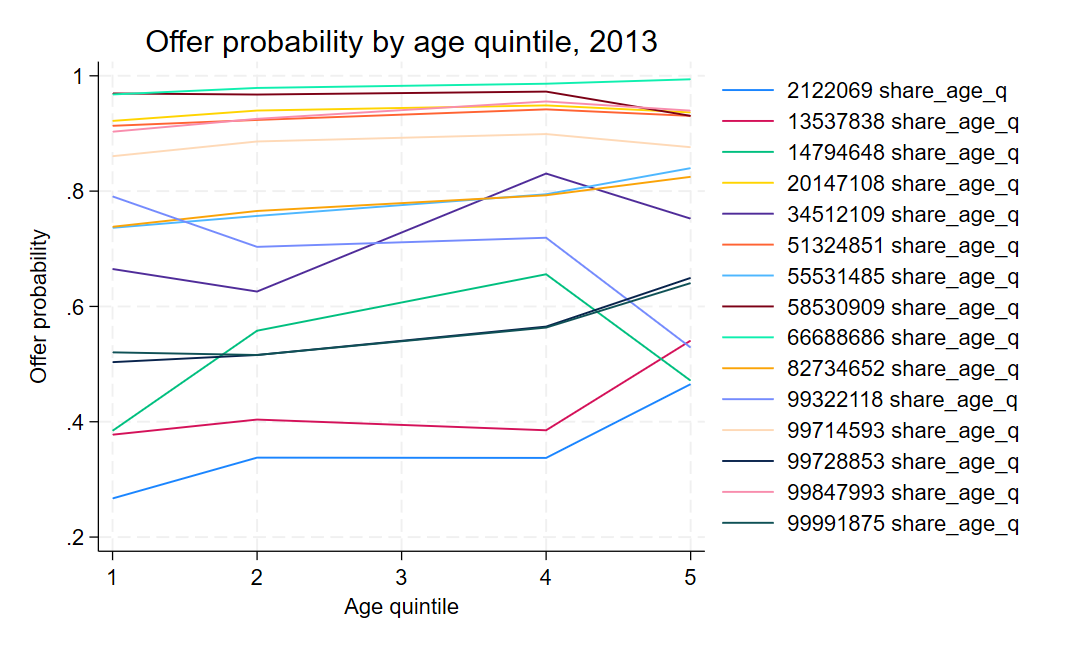
\includegraphics[scale=0.27]{figures/IE3_supply_offerprob_age_q_2013.png}
\end{tabular}
\end{figure}


\begin{figure}[H] 
\caption{}
\label{fig:ie3_16}
\centering{}%
\begin{tabular}{cc}
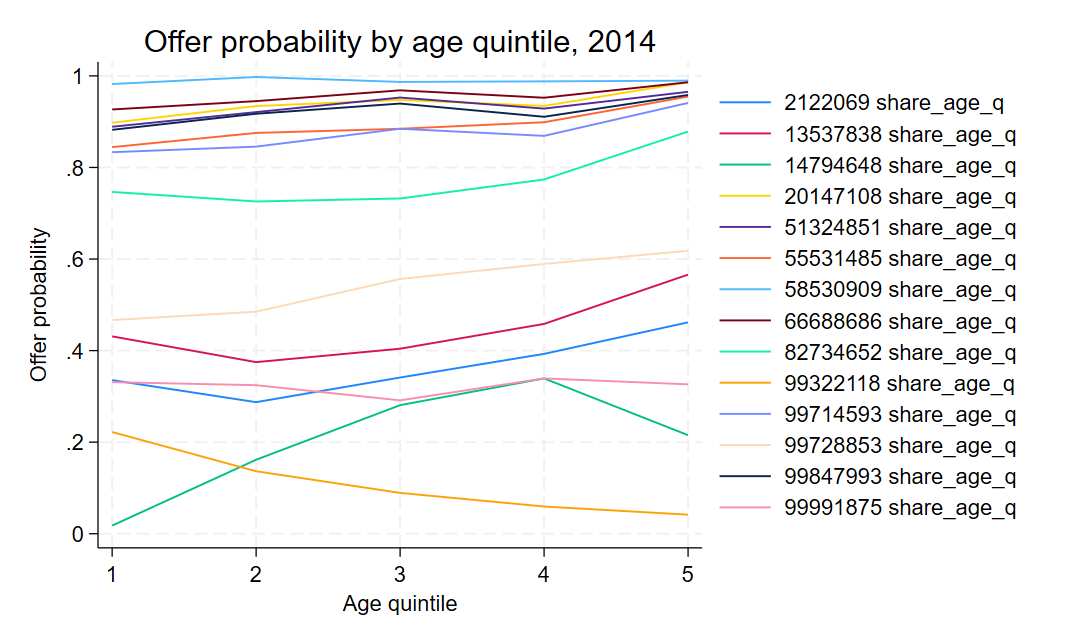
\includegraphics[scale=0.27]{figures/IE3_supply_offerprob_age_q_2014.png} &
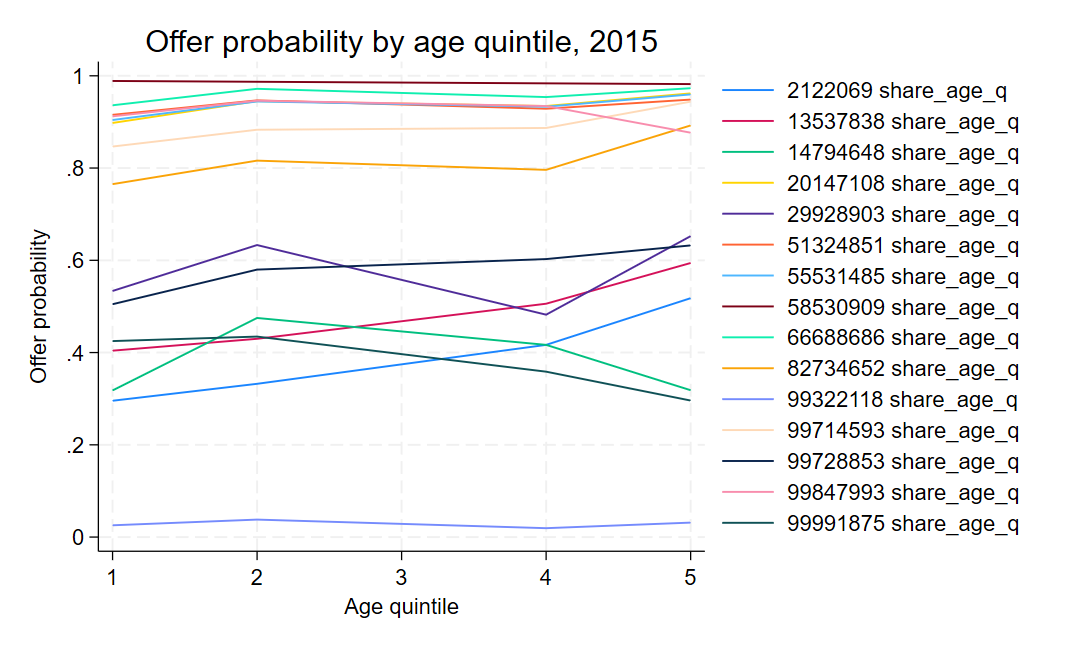
\includegraphics[scale=0.27]{figures/IE3_supply_offerprob_age_q_2015.png}
\end{tabular}
\end{figure}

\end{document}